\documentclass[aspectratio=169]{beamer}

\usetheme{Madrid}
\usecolortheme{default}
\usepackage[utf8]{inputenc}
\usepackage[T1]{fontenc}
\usepackage{booktabs}
\usepackage{graphicx}

\title{Causal Effects of Sea Surface Temperature Anomalies on Extreme Precipitation in the Pacific Northwest (ERA5)}
\author{Pradyumna, Nate, Tiffany, Suditi, Anirudh}
\institute{UCSD DSC 245}
\date{Final Project Presentation}

\begin{document}

\begin{frame}
\titlepage
\end{frame}

\begin{frame}{The Question}
\Large
Under an explicit identification graph, does warm regional SST increase 
ONDJFM 90th-percentile precipitation-extreme risk in the Pacific 
Northwest?
\vspace{0.5cm}

\textbf{Plain Language:} Does regional warm sea surface temperature increase 
the chance of extreme rainfall events in the Pacific Northwest during the 
6 months of fall and winter?
\vspace{0.5cm}

\normalsize
The project is deliberately narrow: it is not a claim about all western-US
precipitation, all winter definitions, or individual storm attribution.
\end{frame}

\begin{frame}{Why This Matters}
\begin{itemize}
    \item \textbf{Decision context:} Seasonal risk screening for Pacific Northwest water
    managers, flood-risk planners, reservoir operators, and emergency preparedness
    offices.
    
    \item \textbf{Use case:} Scenario stress tests, closer monitoring, and risk
    communication when regional SST is warm.
    
    \item \textbf{Limitation:} This is not an operational flood forecast and not an
    attribution tool for individual storms.
\end{itemize}
\end{frame}

\begin{frame}{Data and Estimand}
\begin{columns}

\begin{column}{0.5\linewidth}
    \begin{itemize}
        \item ERA5 monthly reanalysis, 1979--2023.
        \item Pacific Northwest box: 45--50 N, 125--115 W.
        \item \textbf{Treatment}: \texttt{sst\_warm}, regional SST anomaly $\geq 0.5$ K.
        \item \textbf{Outcome}: \texttt{tp\_extreme}, region-specific 90th-percentile
        precipitation extreme.
        \item Season: ONDJFM.
\end{itemize}
\end{column}

\begin{column}{0.5\linewidth}
    
\includegraphics[width=\linewidth]{figures/fig1_domain_map.pdf}
\end{column}

\end{columns}
\end{frame}

\begin{frame}{Methodological Outline}
\begin{itemize}
\setlength{\itemsep}{0.8em}
\item \textbf{Process ERA5 data} into a monthly regional panel with extreme precipitation definitions.
\item \textbf{Time-series causal discovery} (PCMCI+ / VARLiNGAM) identifies candidate dependencies.
\item \textbf{Discovery output is projected} into a lag-0 acyclic causal graph \textbf{for identification}.
\item A fixed (frozen) causal graph defines the \textbf{adjustment set} for \textbf{estimating effects}.
\item \textbf{Causal effects are estimated} using IPW and doubly robust (DR) methods.
\item Robustness, holdout validation, and diagnostics \textbf{assess stability and sensitivity}.
\end{itemize}
\end{frame}


\begin{frame}{Discovery Is Not Identification}
\begin{columns}
\begin{column}{0.5\textwidth}
\begin{itemize}
        \item PCMCI+ and VARLiNGAM summarize time-series dependence.
    \item They are useful discovery inputs, not proof of the true atmospheric DAG.
    \item Identification requires a stated treatment, outcome, population,
adjustment strategy, and assumptions.
    \item We separate discovery output from the graph used for backdoor adjustment.
\end{itemize}
\end{column}

\begin{column}{0.5\textwidth}
\begin{figure}
    \centering
    
\includegraphics[width=1\linewidth]{figures/fig3_pcmci_graphs.pdf}
    \caption{PCMCI+ discovery outputs}
    \label{fig:fig3}
\end{figure}
\end{column}
\end{columns}
\end{frame}

\begin{frame}{Projection Algorithm}
\begin{columns}
    \begin{column}{0.5\textwidth}
        The time-series discovery output is projected into a monthly panel DAG:
\begin{enumerate}
\item Drop self-edges.
\item Keep lag-0 links for the panel graph.
\item Sort candidate links by discovery strength.
\item Greedily add edges while preserving acyclicity.
\item Merge with the domain identification backbone.
\end{enumerate}
    \end{column}
\begin{column}{0.5\textwidth}
\centering
    \textbf{Backbone}
    \vspace{0.2cm}
    %\texttt{nino34 -> z500},
    %\texttt{nino34 -> sst},
    %\texttt{z500 -> tp},
    %\texttt{sst -> tp},
    %\texttt{tp -> tp\_extreme}.
    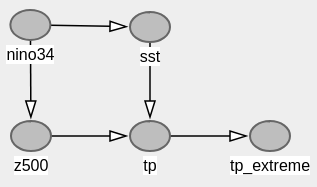
\includegraphics[width=0.8\linewidth]{backbone DAG.png}
\end{column}
\end{columns}

\end{frame}

\begin{frame}{Adjustment Set}
\begin{columns}
    \begin{column}{0.5\textwidth}
        \begin{itemize}
        \item Primary graph-identified adjustment set: \textbf{\{\texttt{z500}\}}.
        \item \textbf{\{\texttt{z500}\}} blocks the large-scale circulation backdoor path in the merged identification graph.
        \item Adding more variables is not automatically better
        \item \textbf{Therefore} larger observed sets are sensitivity checks, not replacements
        for the primary estimand.
\end{itemize}
    \end{column}
    \begin{column}{0.3\textwidth}
        Additional Variables:
        \begin{itemize}
            \item \texttt{nino34}
            \item \texttt{t2m}
            \item \texttt{swvl1} 
        \end{itemize}
        may be ancestors, mediators, descendants, or
        precision variables depending on the assumed graph
    \end{column}
\end{columns}
\end{frame}

\begin{frame}{Main Result}

\includegraphics[width=\linewidth]{figures/fig7_primary_holdout_summary.pdf}
\end{frame}

\begin{frame}{Primary Estimates}
\begin{table}
\centering
\begin{tabular}{lrr}
\toprule
Estimator & Risk difference & 95\% CI \\
\midrule
IPW & 0.146 & [0.026, 0.237] \\
DR & 0.160 & [0.040, 0.245] \\
IPW holdout & 0.180 & [0.016, 0.361] \\
DR holdout & 0.066 & [0.045, 0.085] \\
\bottomrule
\end{tabular}
\end{table}

\vspace{0.2cm}
The full-sample and post-2000 holdout estimates are positive and separated from
zero.

\vspace{0.2cm}
\textbf{DR}: doubly robust, \textbf{IPW}: Inverse propensity reweighting

\end{frame}

\begin{frame}{Holdout Interval Audit}
%\begin{itemize}
%\item Holdout nuisance models are fit on 1979--1999 and evaluated on 2000--2023.
%\item The DR interval is much tighter than IPW: IPW width is 8.7 times DR width.
%\item Explanation: the bootstrap varies evaluation rows while keeping train-fitted nuisance models fixed.
%\item DR is stabilized by its outcome-effect model; IPW remains more sensitive to inverse-propensity weighting.
%\item The tight DR interval is useful, but model-dependent.
%\end{itemize}
Holdout nuisance models are fit on 1979--1999 and evaluated on 2000--2023
\vspace{0.2cm}
\begin{columns}
    \begin{column}{0.5\textwidth}
        \begin{itemize}
        \item The DR interval is much tighter than IPW: \textbf{IPW width is 8.7 times DR width.}
        \item \textbf{Explanation:} the bootstrap varies evaluation rows while keeping train-fitted nuisance models fixed.
        %\item DR is stabilized by its outcome-effect model IPW remains more sensitive to inverse-propensity weighting.
        %\item The tight DR interval is useful, but model-dependent.
        \end{itemize}
    \end{column}
    \begin{column}{0.5\textwidth}
        \begin{itemize}
        \item \textbf{DR} is \textbf{stabilized} by its \textbf{outcome-effect model}
        \item \textbf{IPW} remains \textbf{more sensitive}.
        \item The tight DR interval is useful, but model dependent.
        \end{itemize}
    \end{column}
\end{columns}
\end{frame}

\begin{frame}{Baseline and Sensitivity Checks}
\centering
\begin{minipage}{0.70\textwidth}

\begin{table}
\centering
\small
\begin{tabular}{lrr}
\toprule
Check & Risk difference & 95\% CI \\
\midrule
Crude logistic & 0.094 & [-0.008, 0.205] \\
Graph-adjusted logistic & 0.147 & [0.051, 0.237] \\
Expanded logistic & -0.007 & [-0.105, 0.100] \\
Lagged circulation/ENSO IPW & 0.227 & [0.047, 0.449] \\
Autoregressive \texttt{tp\_lag1} IPW & 0.156 & [0.037, 0.282] \\
\bottomrule
\end{tabular}
\end{table}

\vspace{0.2cm}

\begin{itemize}
    \item The signal is visible in a simple graph-adjusted model
    \item Broad observed adjustment is a real sensitivity concern.
\end{itemize}

\end{minipage}

\end{frame}

\begin{frame}{Negative Results Are Part of the Claim}
\begin{itemize}
\item California: weak/null.
\item Intermountain West: weak/null.
\item Pooled western-US stack: null.
\item NDJF-only seasonal variant: fails sign stability.
\item External MERRA-2/JRA-55 validation: scoped as future work, not claimed.
\end{itemize}
\end{frame}

\begin{frame}{Limitations}
\begin{itemize}
\item Identification depends on the domain backbone and lag-0 projection.
\item Broad observed adjustment has poor overlap and weakens the estimate.
\item Monthly aggregation smooths submonthly storm dynamics.
\item Atmospheric rivers are likely mechanisms behind many PNW extremes, but no
AR covariate is included.
\item ERA5 temporal holdout is not the same as cross-product external
validation.
\end{itemize}
\end{frame}

\begin{frame}{Takeaway}
\Large
Warm regional SST anomalies increase ONDJFM extreme-precipitation risk in the
Pacific Northwest in ERA5 under a frozen identification graph.

\vspace{0.5cm}

\textbf{Plain Language:} Regional warm sea surface temperatures increase 
the chance of extreme rainfall events in the Pacific Northwest during the 
6 months of fall and winter in the ERA5 dataset, under a fixed causal structure.

\vspace{0.5cm}
\normalsize
The claim is narrow, auditable, temporally validated, and explicitly
assumption-sensitive. That is the point of the workflow.
\end{frame}

\end{document}
